\documentclass[12pt]{article}


\usepackage{geometry}
 \geometry{
 a4paper,
 left=20mm,
 right=20mm,
 top=10mm
 }


\usepackage[utf8]{inputenc}
\usepackage{graphicx}

\title{TJV - Architektura podnikových aplikací. Popis jednotlivých vrstev JEE aplikací: klientská vrstva, webová vrstva, vrstva obchodní logiky, EIS vrstva.}
\author{Vastl Martin}

\begin{document}
\maketitle
\author
 
\section{Podnikové aplikace}
Java Enterprise Edition (JEE) je součást platformy Javy určená pro vývoj a provoz podnikových aplikací a informačních systémů. Od podnikové aplikace se očekávají tyto vlastnosti: 

\begin{itemize}
	\item Robustnost, bezpečnost, rozšiřovatelnost a škálovatelnost.
	\item Schopnost obsloužit velké množství klientů.
	\item Pracující s různě velkými a rozličnými daty uloženými v různých datových systémech.
	\item Komunikující s dalšími systémy pomocí definovaných rozhraní.
\end{itemize}
 
Java Enterprise Edition (JEE) definuje 4 vrstvy architektury.
\begin{enumerate}
	\item Klientská vrstva
	\item Webová vrstva
	\item Vrstva obchodní logiky (Business vrstva)
	\item Enterprise Information System (EIS) vrstva
\end{enumerate} 
Java EE platforma se zaměřuje na vývoj ve webové a business vrstvě, které běží na aplikačním serveru. Jelikož tyto dvě vrstvy obvykle běží na stejném stroji, jsou někdy dohromady označovány jako střední vrstva, a proto někdy JEE architekturu nazýváme 3 vrstvou.

\begin{figure}
\centering
	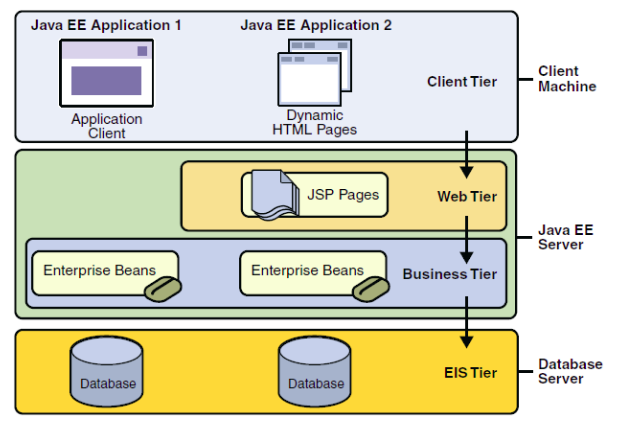
\includegraphics[scale=0.5]{vrstvy.png}
	\caption{Vrstvy architektury.}\label{img:vrstvy}
\end{figure}

\section{Klientská vrstva}
Klientskou vrstvu představuje aplikace, která nemusí být napsána (programována) v Javě. Dva základní typy klientů jsou:
\begin{itemize}
	\item webový prohlížeč, který komunikuje s webovou vrstvou za pomocí HTTP požadavků.
	\item klientská aplikace, která může komunikovat s webovou vrstvou za pomocí HTTP poža\-dav\-ků a nebo na přímo.
\end{itemize} 
Úlohou klienta je zasílat požadavky střední vrstvě, přijímat od ní odpovědi a prezentovat je uživateli.
\begin{figure}
\centering
	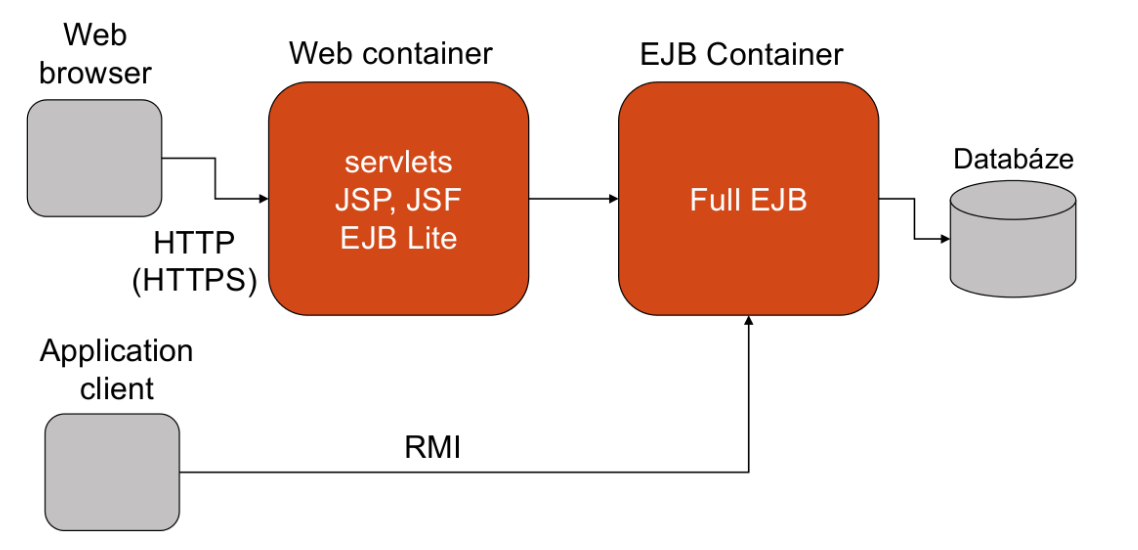
\includegraphics[width=0.8\linewidth]{klient.png}
	\caption{Klient}\label{img:klient}
\end{figure}

\section{Webová vrstva}
Webová vrstva je tvořena servlety, JSP a JSF soubory a případně také JavaBeans komponentami. Tyto komponenty zpracovávají klientské požadavky a generují odpověď, která je následně zaslána do webového prohlížeče klienta. 
Při zpracovávání odpovědi může webová vrstva komunikovat s vrstvou obchodní logiky (business vrstvou) a získávat od ní určité informace. 

\section{Obchodní logika}
Zde leží jádro celé aplikace. Veškerá logika a funkcionalita by měla být uložena v business vrstvě, konkrétně v EJB komponentách. 
EJB komponenty přijímají požadavky od klientské a webové vrstvy a na jejich základě pracují se zdroji z EIS vrstvy. 
Následně zasílají odpověď zpět klientské respektive webové vrstvě. 

\section{EIS vrstva}
Je vrstva sloužící pro persistentní ukládání dat. Jako o EIS hovoříme proto, že z hlediska JEE neřešíme jakého typu data jsou (relační, objektově uložená či získaná z nějakého jiného systému). Pro JEE je důležité zajistit jednotný přístup k těmto datům. To zajišťuje (mimo řady dalších služeb) JNDI (Java Naming and Directory Interface), která zajistí na základě klíčového slova zajistí vyhledání a předání existující konfigurace požadující od serveru. Dále aplikační server zajistí pool připojení a předá připojení aplikaci. Dále se může aplikační server postarat práva jednotlivých uživatelů a stará se o refresh connection a uzavírá a otevírá spojení. Cílem je odstínit programátora obchodní vrstvy o konfigurace a správu jednotlivých datových zdrojů. Předtím než lze použít datový zdroj je nutné, aby byl nainstalován JDBC driver, nastaven connection pool (user, password, název databáze, \ldots) a jdbc zdroj, který je nasměrován na požadovaný connection pool.


 
\end{document}